% This file: 			Draft Compiling New Information and Analysis
% Contributors: 		Pietro Biroli, Daniela Del Boca, Linor Kiknadze, 
%					Yu Kyung Koh, Sylvi Kuperman, Sidharth Moktan, 
%					Chiara Pronzato, Nirali Trevedi, Anna Ziff
% Original date: 		10/3/16
% Project: 			Reggio Evaluation

%Style
\documentclass[12pt]{article}
\usepackage[top=1in, bottom=1in, left=1in, right=1in]{geometry}
\parindent 22pt
\usepackage{fancyhdr}

%Packages
\usepackage{adjustbox}
\usepackage{amsmath}
\usepackage{amsfonts}
\usepackage{amssymb}
\usepackage{bm}
\usepackage[table]{xcolor}
\usepackage{tabu}
\usepackage{makecell}
\usepackage{longtable}
\usepackage{multirow}
\usepackage[normalem]{ulem}
\usepackage{etoolbox}
\usepackage{graphicx}
\usepackage{tabularx}
\usepackage{ragged2e}
\usepackage{booktabs}
\usepackage{caption}
\usepackage{fixltx2e}
\usepackage[para, flushleft]{threeparttablex}
\usepackage[capposition=top]{floatrow}
\usepackage{subcaption}
\usepackage{pdfpages}
\usepackage{pdflscape}
\usepackage{natbib}
\usepackage{bibunits}
\definecolor{maroon}{HTML}{990012}
\usepackage[colorlinks=true,linkcolor=maroon,citecolor=maroon,urlcolor=maroon,anchorcolor=maroon]{hyperref}
\usepackage{marvosym}
\usepackage{makeidx}
\usepackage{tikz}
\usetikzlibrary{shapes}
\usepackage{setspace}
\usepackage{enumerate}
\usepackage{rotating}
\usepackage{epstopdf}
\usepackage[titletoc]{appendix}
\usepackage{framed}
\usepackage{comment}
\usepackage{xr}
\usepackage{titlesec}
\usepackage{footnote}
\usepackage{longtable}
\newlength{\tablewidth}
\setlength{\tablewidth}{9.3in}
\setcounter{secnumdepth}{4}

\titleformat{\paragraph}
{\normalfont\normalsize\bfseries}{\theparagraph}{1em}{}
\titlespacing*{\paragraph}
{0pt}{3.25ex plus 1ex minus .2ex}{1.5ex plus .2ex}
\makeatletter
\pretocmd\start@align
{%
  \let\everycr\CT@everycr
  \CT@start
}{}{}
\apptocmd{\endalign}{\CT@end}{}{}
\makeatother
%Watermark
\usepackage[printwatermark]{xwatermark}
\usepackage{lipsum}
\definecolor{lightgray}{RGB}{220,220,220}
%\newwatermark[allpages,color=lightgray,angle=45,scale=3,xpos=0,ypos=0]{Preliminary Draft}

%Further subsection level
\usepackage{titlesec}
\setcounter{secnumdepth}{4}
\titleformat{\paragraph}
{\normalfont\normalsize\bfseries}{\theparagraph}{1em}{}
\titlespacing*{\paragraph}
{0pt}{3.25ex plus 1ex minus .2ex}{1.5ex plus .2ex}

\setcounter{secnumdepth}{5}
\titleformat{\subparagraph}
{\normalfont\normalsize\bfseries}{\thesubparagraph}{1em}{}
\titlespacing*{\subparagraph}
{0pt}{3.25ex plus 1ex minus .2ex}{1.5ex plus .2ex}

%Functions
\DeclareMathOperator{\cov}{Cov}
\DeclareMathOperator{\var}{Var}
\DeclareMathOperator{\plim}{plim}
\DeclareMathOperator*{\argmin}{arg\,min}
\DeclareMathOperator*{\argmax}{arg\,max}

%Math Environments
\newtheorem{theorem}{Theorem}[section]
\newtheorem{claim}[theorem]{Claim}
\newtheorem{assumption}[theorem]{Assumption}
\newtheorem{definition}[theorem]{Definition}
\newtheorem{hypothesis}[theorem]{Hypothesis}
\newtheorem{property}[theorem]{Property}
\newtheorem{example}[theorem]{Example}
\newtheorem{condition}[theorem]{Condition}
\newtheorem{result}[theorem]{Result}
\newenvironment{proof}{\paragraph{Proof:}}{\hfill$\square$}

%Commands
\newcommand\independent{\protect\mathpalette{\protect\independenT}{\perp}}
\def\independenT#1#2{\mathrel{\rlap{$#1#2$}\mkern2mu{#1#2}}}
\newcommand{\overbar}[1]{\mkern 1.5mu\overline{\mkern-1.5mu#1\mkern-1.5mu}\mkern 1.5mu}
\newcommand{\equald}{\ensuremath{\overset{d}{=}}}
\captionsetup[table]{skip=10pt}
%\makeindex


\newcolumntype{L}[1]{>{\raggedright\let\newline\\\arraybackslash\hspace{0pt}}m{#1}}
\newcolumntype{C}[1]{>{\centering\let\newline\\\arraybackslash\hspace{0pt}}m{#1}}
\newcolumntype{R}[1]{>{\raggedleft\let\newline\\\arraybackslash\hspace{0pt}}m{#1}}



%Logo
%\AddToShipoutPictureBG{%
%  \AtPageUpperLeft{\raisebox{-\height}{\includegraphics[width=1.5cm]{uchicago.png}}}
%}

\newcolumntype{L}[1]{>{\raggedright\let\newline\\\arraybackslash\hspace{0pt}}m{#1}}
\newcolumntype{C}[1]{>{\centering\let\newline\\\arraybackslash\hspace{0pt}}m{#1}}
\newcolumntype{R}[1]{>{\raggedleft\let\newline\\\arraybackslash\hspace{0pt}}m{#1}} 

\newcommand{\mr}{\multirow}
\newcommand{\mc}{\multicolumn}

%\newcommand{\comment}[1]{}


\begin{document}

\title{Evaluation of the Reggio Approach \\ Draft}
\author{Reggio Team}
\date{Original version: October 3, 2016 \\ Current version: \today}
\maketitle

\tableofcontents

\doublespacing

\section{Introduction}
\label{sec:introduction}
Evidence from seminal experiments in early childhood interventions, such as the Perry Preschool Program, demonstrates the potential for early childhood education to improve life-cycle outcomes of disadvantaged individuals \citep{Heckman_Moon_etal_2010_QE, Elango_Hojman_etal_2016_Early-Edu}. There are many early childhood interventions that are widely replicated with little empirical evidence of their effectiveness. One such intervention is the Reggio Approach (RA). Starting in 1963 in Reggio Emilia in Northern Italy, the RA is still implemented in the municipal schools of Reggio Emilia, as well as replicated internationally.\footnote{The official \href{http://www.reggiochildren.it/network/?lang=en}{Reggio Children International Network} is present in 33 countries worldwide. Many other preschools around the world are ``inspired'' by the Reggio Approach but they are not officially part of these network.}

This paper presents an evaluation of the Reggio Approach early childhood education system in Reggio Emilia, which includes infant-toddler centers (ages 0-3) and preschools (ages 3-6). The Reggio Approach is administrated through the municipal government of Reggio Emilia. Other early childhood education options include state preschools and private infant-toddler centers and preschools. We have collected data on individuals who have attended all these types of early childhood education as well as those who were informally taken care of outside of a center setting. 

Our sample includes individuals across five age cohorts: three cohorts of adults, one cohort of adolescents, and one cohort of children in their first year of elementary school. The individuals are not only from Reggio Emilia, but also from Padova and Parma, two cities that are similar to Reggio Emilia along several dimensions but have different preschool systems. Table~\ref{tab:overview} presents an overview of the structure of the data.

% placeholder
\begin{table}[H]
\centering
\begin{threeparttable}
\caption{Dataset Structure} \label{tab:overview}
	\begin{tabular}{lcc}
\toprule
Cohort 			& Years of Birth 	& Age at Interview \\ \midrule
Adults (50s)	  	& 1954-1959 		& 54-60 \\
Adults (40s)	   	& 1969-1970		& 43	\\
Adults (30s)    		& 1980-1981		& 32    \\
Adolescents 	   	& 1994			& 18 	\\
Children 	   		& 2006			& 6 \\ 
\bottomrule 
\end{tabular}
\begin{tablenotes}
Note:
\end{tablenotes}
\end{threeparttable}
\end{table}

Evaluating the Reggio Approach presents several challenges, given the non-experimental nature of the program. The Reggio Approach preschool system was introduced in 1963, grew over the decades, and now has infrastructure to teach educators about the Reggio Approach. Therefore, he evaluation strategy has to account for potential changes in treatment over time, lack of well defined control group, and potential spillover of the Reggio Approach into other programs attended by individuals in the data. 

This analysis \ldots We find \ldots

In Section~\ref{sec:eceexperiences}, we describe the Reggio Approach and the other early childhood education experiences in the three cities focusing on administrative changes that might have led to a diffusion of aspects of the Reggio Approach. We also present an overview of the demographic aspects of Reggio Emilia, Parma, and Padova that contextualize the differences in approaches to early childhood education. Section~\ref{sec:data} describes the data in more detail and discusses the outcome variables that are available for the different cohorts. Section~\ref{sec:methodology} discusses the methodology we employ to produce the results discussed in Section~\ref{sec:results}. Section~\ref{sec:conclusion} concludes.

\section{Early Childhood Education Experiences}
\label{sec:eceexperiences}

We first present some demographic characteristics of Reggio Emilia, Parma, and Padova, and discuss some social trends to contextualize the early childhood education options in the three cities. Then, we describe the Reggio Approach, which we consider to be the treatment in this evaluation. Because the group of individuals who did not receive this treatment did not uniformly stay at home or receive a homogenous alternative early childhood education experience, we also document the curricular and programmatic elements of these alternative programs.

\subsection{Background on Cities}
\label{sec:backgroundcities}

\textbf{[AZ: Include graphs and information from Linor]}

\subsection{Types of Early Childhood Education in Italy}

In Italy, the responsibilities for the funding and provision of early childhood care and education are as follows: the state passes laws, defines educational aims, and provides the majority of funding for schools to regions through the Health Ministry. Each region may pass laws regarding the organization and basic planning of centers in that region. Municipalities organize and run the schools \citep{Becchi-Ferrari_1990_Pub-Inf-Centres-Italy}. 

Municipalities are further enabled to set eligibility criteria for public early childhood education. Selection criteria are similar across municipalities, however, the weighting of distinct family characteristics varies \citep{Del-Boca-etal_2016_CESifo-ES}. State preschools are free to all families, but charge for meals and transportation. Fees to attend municipal schools vary; about half of municipalities provide free early childcare while others are offered on a sliding scale.

The Catholic Church offers the majority of private religious early childhood programs. Tuition is the family's responsibility, depending on income and amount of state subsidy available as decided by the municipality. Private secular early childhood programs tend to be the sole responsibility of the family \citep{Hohnerlein_2009_Paradox-Public-Preschools}.

To summarize, early childhood education is publicly provided by the municipality or the state, and privately provided by religious institutions or secular ones. \textbf{[AZ: Maybe include some table or figure tabulating attendance to these types in the data?]}

\subsection{Reggio Approach}
\textbf{[AZ: This section needs more citations. I also moved things around so please double check that you agree with everything!]}

The Reggio Approach is a form of progressive early childhood education designed by Loris Malaguzzi, an educator influenced by the educational practices and psychological theories of Ciari, Dewey, Piaget, Erikson, Vygotsky, Bronfenbrenner, Kagan, and Gardner. \textbf{[AZ: Perhaps we should briefly describe some of the theories and cite these individuals instead of listing the individuals?} The Reggio Approach emerged from political conflict between the secular and communist left and the religious and conservative right. Malaguzzi was one of several left-wing educators within the region of Emilia Romagna. Under the guidance of Malaguzzi, Reggio Emilia opened its first preschool in 1963 for children aged 3-6 years. In 1965 \textbf{[AZ: Should this be 1971?]}, Reggio Emilia opened the first infant-toddler center for children aged 3 months to 3 years. The Reggio Emilia municipal system with this progressive model preceded reforms in the 60s and 70s that established state-run infant-toddler centers and preschools.

In the Reggio Approach, preschool-aged children are active learners, or ``researchers." Curriculum is viewed as an ongoing, collaborative project, in contrast to a pre-defined set of learning activities. Children's developing knowledge is expressed in creative forms and documented in portfolios that are subsequently shared with the parents and children. 

The Reggio Approach infant-toddler center opens at 8am. Families can choose three options for pick-up: 1 p.m. (part-day), 4 p.m. (full-time), and until 6:20 p.m. (extended day). Teachers in the infant-toddler center generally have lower initial training and receive less pay. The atelierista is not part of the infant-toddler center, but in Reggio Emilia, teachers are trained by atelieristas from the preschools. In contrast to the Reggio Approach preschool, teachers are assigned to children in single-year increments \citep{Cagliari-etal-eds_2016_BOOK_Loris-Malaguzzi,Giudici-Nicolosi_2014_Reggio-Approach}.

Preschools are open five full-time days per week from September through July \citep{Giudici-Nicolosi_2014_Reggio-Approach}. The educative team is assigned specialized roles. Each class is led by two full-time co-teachers, and each school site has one full-time atelierista, an instructor with a background in visual arts. Auxiliary site staff, such as cooks and janitors, are considered members of the educative staff and are included in all trainings. A pedagogista, with a higher degree in psychology or education, is assigned to support professional development for the educative staff of approximately 4-5 schools. In addition to having an atelierista, each school is equipped with an in-house kitchen and is has an open interior design.  

Teachers remain with the same group of children for three consecutive years, and thus have extended time to know each child and their families. There is no predetermined curriculum enacted by educators in that there are no distinct timelines or institutionally-prescribed content knowledge that educators must convey to achieve ``school readiness." In contrast, educators, children (and sometimes families) collaborate to define a question or topic and pursue research that is not constrained by a predetermined timeline. Teachers observe, scaffold learning, and engage children in discussion. Children demonstrate their emerging knowledge through creative visual media, aided by the atelierista. Teachers document each child's development in a portfolio---a collection of work---which is reviewed and discussed with children and parents over the year. 

\subsection{Other Early Childhood Education Experiences}

Municipal early childhood education programs in Reggio Emilia, Parma and Padova differ in certain aspects of program administration, environmental features, and pedagogical methods. We discuss these differences below. 

\subsubsection{Parma}

Published literature documenting the Parma municipal early childhood system in detail is scarce. Carolyn Pope Edwards suggests that municipal schools in Parma are parallel to those of Reggio Emilia.\footnote{Kuperman, Interview with Carolyn Pope Edwards, 2016. See \citet{Edwards-etal-eds_1998_Hundred-Languages}.} 

As of 2001, 16 infant-toddler centers were offered throughout the municipality. The administration of these centers are managed by a director of services for children under 3 years of age. Pedagogical coordinators perform both administrative and professional development roles. Assigned to a specific set of infant-toddler centers, they meet twice each month with all site teachers collectively for shared reflection, on-site supervision, and to promote relationships with families. The city director meets biweekly with all pedagogical coordinators for overall planning. University professors or administrators from other municipalities provide professional development in the form of continuing education \citep{Terzi-Cantarelli_2001_Parma}.

In contrast to pre-fabricated preschool centers, Parma's infant-toddler centers are intentionally designed in the context of an apartment. \citet{Terzi-Cantarelli_2001_Parma} report mixed-age classes that include 18 total children from 13 months to 3 years in a single section, led by two teachers (9:1 child-teacher ratio). To accommodate parents, infant-toddler centers open at 7:30pm and offer 3 pick-up times: 2 p.m. (short-day), 3:30 p.m. (normal-day), or 5 p.m. (extended-day). Classrooms can be organized by single-age groups (e.g., 5-12 months, 12-24 months, and 24-36 months) or by mixed-age groups (e.g.,12-36 months) \citep{Majorano-etal_2009_CC-in-P}.

\textbf{[AZ: Information on preschool in Parma]}

\subsubsection{Padova}
Padova is located in the relatively more religious and politically diverse region of Veneto. Compared to Reggio Emilia and Parma, its municipal early childhood education system is smaller and it has a higher number of private religious programs. 

In 1989, the region of Veneto reported a total provision of childcare slots for 3.9\% of its infant-toddler population. In contrast, the region of Emilia Romagna reported a provision of infant-toddler childcare for 15.6\% of its population. The practice of professional development trainings for early childhood staff in Veneto first began in 1986. \textbf{[AZ: citation?]}

The Catholic Church offers the majority of private religious early childhood programs; tuition is the family's responsibility, depending on income and amount of state subsidy available as decided by the municipality \citep{Hohnerlein_2009_Paradox-Public-Preschools}.  A major concern of the Catholic Church in Italy is equity and parity of state funding for private schools.\footnote{In 2005, funding for state and private schools differed greatly. Authorized private schools received a state contribution for pre-primary schools (ages 2-6 years), while funding for private primary schools (ages 6-11 years) was at 15.5\% the rate of public primary schools. Private secondary schools (ages 11-18 years) received no state funding. \textbf{[AZ: citation?]}}

Prior to March 2000, state funding for private schools reflected a 1947 constitutional clause that non-state schools could operate ``without financial burdens on the state.'' Private schools were thus considered options only for affluent families that could afford the tuition expense. \textbf{[AZ: citation?]}

\section{Data}
\label{sec:data}

%Describe survey data collection process and provide more details about the sample
%Discuss selection issues. Present baseline characteristics of those who attended the different types.
%Briefly mention how we select control variables

The sample was collected from the population of individuals in Reggio Emilia, Parma, and Padova who were born in the year ranges of the five cohorts.  These individuals were collected from the population registries in each of the cities. The sample was then restricted to those individuals who live in the same city in which they were raised. All cohorts except the youngest one were restricted to individuals who are Italian citizens. In contrast, the youngest cohort includes an oversampling of immigrant children. The sample from Reggio Emilia, across all cohorts, includes an oversampling of those who attended municipal schools, as this is considered the treatment.

Of the reference sample, 7,109 individuals were randomly selected. Of these, 4,019 completed interviews, resulting in a response rate of 56.5\%. Figure~\ref{fig:sample} presents an overview of the sample highlighting those who attended a Reggio Approach preschool. Table~\ref{tab:sample} provides a detailed tabulation of the sample by city, cohort, and school type.

\begin{figure}[H]
\begin{center}
\caption{Overview of Sample}\label{fig:sample}
	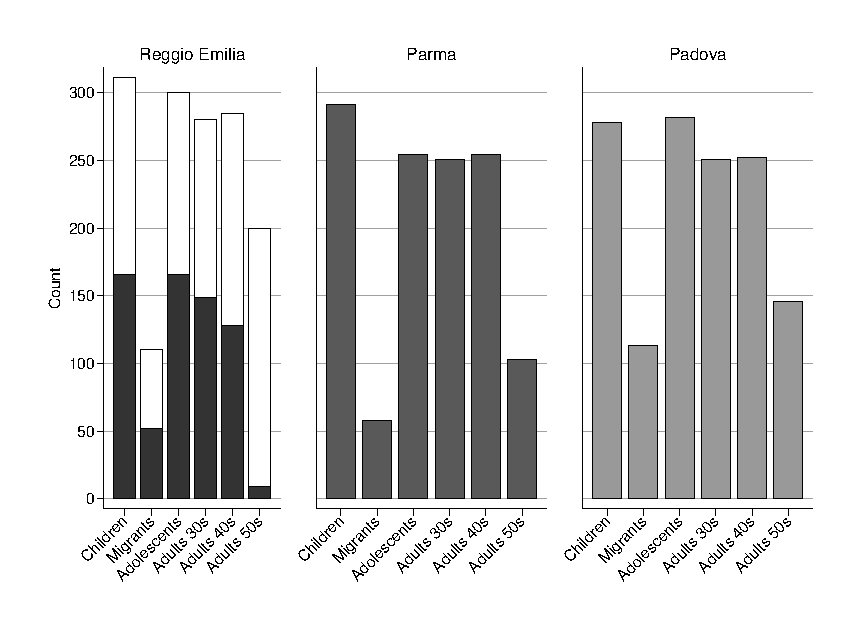
\includegraphics[width=.9\textwidth]{output/sample.eps}
\end{center}
\raggedright
Note: This figure displays the number of individuals by cohort and city. The bars for Reggio Emilia differentiate between those who attended municipal preschool (black bars) and those who did not (white bars). 
\end{figure}

\begin{table}[H]
\centering
\scalebox{0.7}{
\begin{threeparttable}
	\caption{Sample by Cohort, City, and School Type}\label{tab:sample}
	\begin{tabular}{l*{15}{c}}
\toprule
            &\mc{5}{c}{Reggio Emilia: 1,471}   &     \mc{5}{c}{ Parma: 1,198}       &      \mc{5}{c}{Padova: 1,305}      \\
           \cmidrule(lr){2-6} \cmidrule(lr){7-11} \cmidrule(lr){12-16} 
      &        None&       Muni.&       State&      Relig.&       Priv.&        None&       Muni.&       State&      Relig.&       Priv.&        None&       Muni.&       State&      Relig.&       Priv.\\
\midrule
Children    &           2&         166&          45&          92&           5&           6&         154&          43&        77&           9&           2&          82&          40&         141&          12\\
Migrants    &           4&          52&          37&          14&           1&           4&          35&          10&          	3&           6&           5&          36&          47&          23&           1\\
Adolescents &           7&         166&          22&          96&           6&           4&         116&          43&     82&           6&           1&          93&          47&         131&           6\\
Adults 30    &          57&         149&          31&          40&           1&          44&          98&          51&        50&          5&       47&         35&         26&            140&    1 \\
Adults 40    &          80&         128&          17&          52&           5&         116&          52&          26&       55&          1&        75&      27 &            24&            123&  0 \\
Adults 50    &         147&           9&          10&          28&           2&          72&          12&           7&          11&           0 &        57&      11 &           2 &           68&    2 \\
\midrule
	       &         297&         670&         162&         322&          20&         246&         467&   180&    278&          27&      187&      284 &            186&        626& 22  \\
\bottomrule
\end{tabular}


\begin{tablenotes}
Note: This table shows the sample size by city, cohort, and school type. These numbers do not include individuals with an unidentified preschool type. In the whole sample, there are 45 individuals with unidentified preschool type. None: no preschool; Muni.: municipal preschool;  State: state preschool; Relig.: religious preschool; Priv.: private preschool.
\end{tablenotes}
\end{threeparttable}
}
\end{table}

The structure of the cohorts allows us to study the effects of the Reggio Approach at different points throughout the life cycle. The youngest cohort of children were interviewed when they entered primary school, the adolescent cohort when they ended compulsory schooling, and the adult cohorts capture different points of engagement in the labor market and familial decisions. This cohort structure also allows us to evaluate the Reggio Approach compared to the alternative early childhood experiences as they evolved over time.

Separate questionnaires were administered to the children, adolescents, and adults, as well as to the caregivers of the children and adolescents. The questionnaires included items about early childhood experiences, family structure, education, interaction with other ethnicities, and measures cognitive and social-emotional skills. The questionnaires for adults additionally included items about occupation, income, and life satisfaction. 

\section{Methodology}
\label{sec:methodology}
For each of the following methods, we should describe them but also connect them to a policy-relevant interpretation.

\begin{itemize}
\item Baseline OLS comparing broader groups (RA vs. others in Reggio, RA vs. all others, RA vs. none for younger cohorts)
\item Baseline OLS disaggregated
\item Difference in difference fixing different axes
\item IV? 
\end{itemize}

\section{Empirical Results}
\label{sec:results}

\subsection{Possibility of Diffusion}
\label{sec:diffusion}

\textbf{[AZ: The below paragraphs were taken from different areas, but we should develop this into a more cohesive section]}

From 1963 to 1984, Malaguzzi oversaw the early childhood municipal system in Reggio Emilia. He also served as director in nearby Modena until 1974 \citep{Cagliari-etal-eds_2016_BOOK_Loris-Malaguzzi}. In 1994, the Reggio Children organization was founded to promote the international implementation of the Reggio Approach. While Reggio Emilia's 1963 site was the first to open, the cities of Bologna, Modena, Parma, and Pistoia helped incite a ``municipal school revolution" in northern Italy \citep{Hohnerlein_2015_Development-and-Diffusion}. 

There is a long history of political---and pedagogical---conflict between the Catholic Church and municipalities in the Emilia Romagna region such as Reggio Emilia and Parma. Following World War II, the prevailing political party in Italy was the centrist \textit{Democrazia Cristiana}. The Catholic Church ``controlled virtually all'' early childcare centers and the institutions that provided teacher training; in 1955, reports suggest 60\% of Italian children under 6 years of age attended ``confessional \textit{scoule materne}'' \citep{Hohnerlein_2015_Development-and-Diffusion}. After 1963, the \textit{Democrazia Cristiana} lost its absolute majority, and an increasingly secular and center-left government began to assume power \citep{Hohnerlein_2009_Paradox-Public-Preschools}. In 1974, following the 1968 and 1971 state laws mandating access to educational childcare for children under age 6, the Catholic Church established the Italian Federation of Catholic Preschools (FISM) to oversee national operations of its own system of early childhood programs. Between 1981 and 1998, the number of municipal and state \textit{scuole dell'infanzia} increased; enrollment in private-religious preschools dropped from 57.7\% to 42.4\%.

Tables~\ref{tab:comparisonRE} through \ref{tab:comparisonPad} present information related to the curricular and programmatic elements of preschool in Reggio Emilia, Parma, and Padova during the time the cohorts would have attended the schools. Each table represents information for one city. The tables are further subdivided by school type. To understand how these school types relate to the Reggio Approach (Reggio Emilia municipal schools), ten components of the Reggio Approach are listed for each school type by city and cohort. 

The selected components of the Reggio Approach are as follows. See \citet{Rinaldi_2006_ReggioEmilia_BOOK,Giudici-Nicolosi_2014_Reggio-Approach, Cagliari-etal-eds_2016_BOOK_Loris-Malaguzzi} for more information.
\begin{description}
\item[Eligibility priority.] Priority of enrollment is given to single-parent families and children with disabilities.
\item[Teaching Staff hours] Teaching staff work 36 hours per week, of which 3 hours are set aside weekly to interact with families, document children's learning, and participate in professional development.
\item[Two Co-teachers per class of homogenous age.] Two co-teachers per classroom are assigned to incoming 3-year-olds and their families, and remain for the next three years with the same cohort.
\item[Atelierista.] Presence of an on-site, full-time atelierista, with training in visual arts. The Reggio Approach uses visual arts as a creative medium through which children both learn content and demonstrate new knowledge as ``100 Languages."
\item[Pedagogista.] The assignment of a pedagogista, with a higher degree in education or psychology and teaching experience, to mentor the educational and auxiliary staff of 4-5 school sites on a bi-weekly basis, offer ongoing professional development, and improve family-school relations.
\item[Project-based learning.] There is no curriculum with pre-determined expectations for children to acquire specific content knowledge. Instead small groups (4-6 children) engage in research projects to investigate topics that are collaboratively selected by educators, parents, and children. 
\item[Atelier and Environment.] Presence of an atelier (arts-based laboratory/library/classroom), an open floor plan, extensive natural light, and natural furnishings and decorative materials.
\item[Documentation.] Teachers document children's individual and collective growth in portfolios that are shared with parents. Portfolios are reviewed with children to demonstrate growth and development.
\item[Meals prepared in on-site kitchen.] Presence of an internal kitchen in the school site that is used both to prepare meals and for instructional purposes.
\item[Religious teaching.] Religious teaching is \textbf{not} part of the Reggio Approach. This variable is included to compare with other programs that do contain Religious components.
\end{description}

The symbols of the table are as follows: \checkmark\ indicates that the school type for the corresponding city and cohort had that component; $\times$ indicates that the school type did not have that component; $\sim$ indicates that some of the schools within that school type had that component; n/a indicates that the school type was not available for the specified cohort and city; a blank space indicates that we are still compiling information to determine the presence of that component.
\singlespacing

\newgeometry{top=.5in, bottom=.5in, left=.6in, right=.6in}
\begin{table}[htb]
\centering
\scriptsize
\begin{threeparttable}
\caption{Comparison of Different School Types to Reggio Approach, Reggio Emilia}\label{tab:comparisonRE}
	\begin{tabular}{ c l |  c  c  c c c }
\toprule
 & & \rotatebox{90}{Children} & \rotatebox{90}{Adolescents}  & \rotatebox{90}{Adults 30s} & \rotatebox{90}{Adults 40s}  & \rotatebox{90}{Adults 50s} \\
\midrule
\multirow{19}{*}{Municipal$^1$}	&	Eligibility priority	&	\checkmark	&	\checkmark	&	\checkmark	&	\checkmark	&	n/a	\\
	\cmidrule{2-7}												
	&	Staff hours/professional dev.	&	\checkmark	&	\checkmark	&		&		&	n/a	\\
	\cmidrule{2-7}												
	&	2 co-teachers/homogenous age	&	\checkmark	&	\checkmark	&	\checkmark	&	\checkmark	&	n/a	\\
	\cmidrule{2-7}												
	&	Atelierista	&	\checkmark	&	\checkmark	&	\checkmark	&	\checkmark	&	n/a	\\
	\cmidrule{2-7}												
	&	Pedagogista	&	\checkmark	&	\checkmark	&	\checkmark	&	\checkmark	&	n/a	\\
	\cmidrule{2-7}												
	&	Project-based learning	&	\checkmark	&	\checkmark	&	\checkmark	&	\checkmark	&	n/a	\\
	\cmidrule{2-7}												
	&	Atelier/Environment	&	\checkmark	&	\checkmark	&	\checkmark	&	\checkmark	&	n/a	\\
	\cmidrule{2-7}												
	&	Documentation	&	\checkmark	&	\checkmark	&	\checkmark	&	\checkmark	&	n/a	\\
	\cmidrule{2-7}												
	&	Meals prepared on-site/kitchen	&	\checkmark	&	\checkmark	&	\checkmark	&	\checkmark	&	n/a	\\
	\cmidrule{2-7}												
	&	Religious teaching	&	$\times$	&	$\times$	&	$\times$	&	$\times$	&	n/a	\\
	\midrule												
\multirow{19}{*}{Municipal-affiliated$^{2,3}$}	&	Eligibility priority	&	\checkmark	&	n/a	&	n/a	&	n/a	&	n/a	\\
	\cmidrule{2-7}												
	&	Staff hours/professional dev.	&		&	n/a	&	n/a	&	n/a	&	n/a	\\
	\cmidrule{2-7}												
	&	2 co-teachers/homogenous age	&		&	n/a	&	n/a	&	n/a	&	n/a	\\
	\cmidrule{2-7}												
	&	Atelierista	&	\checkmark	&	n/a	&	n/a	&	n/a	&	n/a	\\
	\cmidrule{2-7}												
	&	Pedagogista	&		&	n/a	&	n/a	&	n/a	&	n/a	\\
	\cmidrule{2-7}												
	&	Project-based learning	&		&	n/a	&	n/a	&	n/a	&	n/a	\\
	\cmidrule{2-7}												
	&	Atelier/Environment	&	$\sim$	&	n/a	&	n/a	&	n/a	&	n/a	\\
	\cmidrule{2-7}												
	&	Documentation	&		&	n/a	&	n/a	&	n/a	&	n/a	\\
	\cmidrule{2-7}												
	&	Meals prepared on-site/kitchen	&		&	n/a	&	n/a	&	n/a	&	n/a	\\
	\cmidrule{2-7}												
	&	Religious teaching	&		&		&		&		&	n/a	\\
	\midrule												
\multirow{19}{*}{State}	&	Eligibility priority	&	\checkmark	&		&		&	\checkmark	&	n/a	\\
	\cmidrule{2-7}												
	&	Staff hours/professional dev.	&	$\times$	&		&		&	$\times$	&	n/a	\\
	\cmidrule{2-7}												
	&	2 co-teachers/homogenous age	&	$\sim$	&		&		&		&	n/a	\\
	\cmidrule{2-7}												
	&	Atelierista	&	$\times$	&		&		&	$\times$	&	n/a	\\
	\cmidrule{2-7}												
	&	Pedagogista	&	\checkmark	&		&		&		&	n/a	\\
	\cmidrule{2-7}												
	&	Project-based learning	&	$\times$	&		&		&	$\times$	&	n/a	\\
	\cmidrule{2-7}												
	&	Atelier/Environment	&	$\times$	&		&		&		&	n/a	\\
	\cmidrule{2-7}												
	&	Documentation	&	\checkmark	&		&		&		&	n/a	\\
	\cmidrule{2-7}												
	&	Meals prepared on-site/kitchen	&	$\times$	&		&		&		&	n/a	\\
	\cmidrule{2-7}												
	&	Religious teaching	&	\checkmark	&	\checkmark	&	\checkmark	&	\checkmark	&	n/a	\\
	\midrule												
\multirow{19}{*}{Religious}	&	Eligibility priority	&	$\times$	&		&		&		&		\\
	\cmidrule{2-7}												
	&	Staff hours/professional dev.	&		&		&		&		&	$\times$	\\
	\cmidrule{2-7}												
	&	2 co-teachers/homogenous age	&	$\times$	&		&		&		&	$\times$	\\
	\cmidrule{2-7}												
	&	Atelierista	&	$\times$	&		&		&		&	$\times$	\\
	\cmidrule{2-7}												
	&	Pedagogista	&	\checkmark	&		&		&		&	$\times$	\\
	\cmidrule{2-7}												
	&	Project-based learning	&		&		&		&		&	$\times$	\\
	\cmidrule{2-7}												
	&	Atelier/Environment	&		&		&		&		&	$\times$	\\
	\cmidrule{2-7}												
	&	Documentation	&		&		&		&		&	$\times$	\\
	\cmidrule{2-7}												
	&	Meals prepared on-site/kitchen	&	$\times$	&		&		&		&	\\
	\cmidrule{2-7}												
	&	Religious teaching	&	\checkmark	&	\checkmark	&	\checkmark	&	\checkmark	&	\checkmark	\\
\bottomrule
\end{tabular}
\begin{tablenotes}
\item Note: (1) See \citet{Rinaldi_2006_ReggioEmilia_BOOK,Giudici-Nicolosi_2014_Reggio-Approach, Cagliari-etal-eds_2016_BOOK_Loris-Malaguzzi}. (2) In 1999 and 2001, the municipality of Reggio Emilia integrated two non-profit cooperatives to expand its services. These schools offer a number of childcare slots according to municipal regulations and are overseen by the municipal pedagogical team \citep{Reggio_2008_Brochure}. (3) See \citet{Giudici-Nicolosi_2014_Reggio-Approach}.
\end{tablenotes}
\end{threeparttable}
\end{table}

\begin{table}[htb]
\centering
\scriptsize
\scalebox{.8}[.8]{
\begin{threeparttable}
\caption{Comparison of Different School Types to Reggio Approach, Parma}\label{tab:comparisonPar}
	\begin{tabular}{ c l |  c  c  c c c }
\toprule
 & & \rotatebox{90}{Children} & \rotatebox{90}{Adolescents}  & \rotatebox{90}{Adults 30s} & \rotatebox{90}{Adults 40s}  & \rotatebox{90}{Adults 50s} \\
\midrule
\multirow{19}{*}{Municipal$^4$}	&	Eligibility priority	&	\checkmark	&		&		&		&	n/a	\\
	\cmidrule{2-7}												
	&	Staff hours/professional dev.	&	\checkmark	&		&		&		&	n/a	\\
	\cmidrule{2-7}												
	&	2 co-teachers/homogenous age	&	$\times$	&		&		&		&	n/a	\\
	\cmidrule{2-7}												
	&	Atelierista	&	$\times$	&		&		&		&	n/a	\\
	\cmidrule{2-7}												
	&	Pedagogista	&	\checkmark	&		&		&		&	n/a	\\
	\cmidrule{2-7}												
	&	Project-based learning	&		&		&		&		&	n/a	\\
	\cmidrule{2-7}												
	&	Atelier/Environment	&		&		&		&		&	n/a	\\
	\cmidrule{2-7}												
	&	Documentation	&	\checkmark	&		&		&		&	n/a	\\
	\cmidrule{2-7}												
	&	Meals prepared on-site/kitchen	&	$\times$	&	$\times$	&		&		&	n/a	\\
	\cmidrule{2-7}												
	&	Religious teaching	&		&		&		&		&	n/a	\\
	\midrule												
\multirow{19}{*}{Municipal participatory managed$^5$}	&	Eligibility priority	&		&		&		&		&	n/a	\\
	\cmidrule{2-7}												
													
	&	Staff hours/professional dev.	&		&		&		&		&	n/a	\\
	\cmidrule{2-7}												
	&	2 co-teachers/homogenous age	&	$\times$	&		&		&		&	n/a	\\
	\cmidrule{2-7}												
	&	Atelierista	&		&		&		&		&	n/a	\\
	\cmidrule{2-7}												
	&	Pedagogista	&		&		&		&		&	n/a	\\
	\cmidrule{2-7}												
	&	Project-based learning	&		&		&		&		&	n/a	\\
	\cmidrule{2-7}												
	&	Atelier/Environment	&		&		&		&		&	n/a	\\
	\cmidrule{2-7}												
	&	Documentation	&		&		&		&		&	n/a	\\
	\cmidrule{2-7}												
	&	Meals prepared on-site/kitchen	&	$\times$	&	$\times$	&		&		&	n/a	\\
	\cmidrule{2-7}												
	&	Religious teaching	&		&		&		&		&	n/a	\\
	\midrule												
\multirow{19}{*}{State}	&	Eligibility priority	&	\checkmark	&		&		&		&	n/a	\\
	\cmidrule{2-7}												
	&	Staff hours/professional dev.	&	$\times$	&		&		&		&	n/a	\\
	\cmidrule{2-7}												
	&	2 co-teachers/homogenous age	&		&		&		&		&	n/a	\\
	\cmidrule{2-7}												
	&	Atelierista	&	$\times$	&		&		&		&	n/a	\\
	\cmidrule{2-7}												
	&	Pedagogista	&	\checkmark	&		&		&		&	n/a	\\
	\cmidrule{2-7}												
	&	Project-based learning	&	$\times$	&		&		&		&	n/a	\\
	\cmidrule{2-7}												
	&	Atelier/Environment	&	$\times$	&		&		&		&	n/a	\\
	\cmidrule{2-7}												
	&	Documentation	&	\checkmark	&		&		&		&	n/a	\\
	\cmidrule{2-7}												
	&	Meals prepared on-site/kitchen	&	$\times$	&	$\times$	&		&		&	n/a	\\
	\cmidrule{2-7}												
	&	Religious teaching	&		&		&		&		&	n/a	\\
	\midrule												
\multirow{19}{*}{Municipal-affiliated/Private}	&	Eligibility priority	&		&		&		&		&		\\
	\cmidrule{2-7}												
	&	Staff hours/professional dev.	&		&		&		&		&		\\
	\cmidrule{2-7}												
	&	2 co-teachers/homogenous age	&		&		&		&		&		\\
	\cmidrule{2-7}												
	&	Atelierista	&		&		&		&		&		\\
	\cmidrule{2-7}												
	&	Pedagogista	&		&		&		&		&		\\
	\cmidrule{2-7}												
	&	Project-based learning	&		&		&		&		&		\\
	\cmidrule{2-7}												
	&	Atelier/Environment	&		&		&		&		&		\\
	\cmidrule{2-7}												
	&	Documentation	&		&		&		&		&		\\
	\cmidrule{2-7}												
	&	Meals prepared on-site/kitchen	&		&		&		&		&		\\
	\cmidrule{2-7}												
	&	Religious teaching	&		&		&		&		&		\\
	\midrule												
\multirow{19}{*}{Religious}	&	Eligibility priority	&	$\times$	&		&		&		&		\\
	\cmidrule{2-7}												
	&	Staff hours/professional dev.	&	\checkmark	&		&		&		&		\\
	\cmidrule{2-7}												
	&	2 co-teachers/homogenous age	&		&		&		&		&		\\
	\cmidrule{2-7}												
	&	Atelierista	&		&		&		&		&		\\
	\cmidrule{2-7}												
	&	Pedagogista	&	\checkmark	&		&		&		&		\\
	\cmidrule{2-7}												
	&	Project-based learning	&		&		&		&		&		\\
	\cmidrule{2-7}												
	&	Atelier/Environment	&		&		&		&		&		\\
	\cmidrule{2-7}												
	&	Documentation	&	\checkmark	&		&		&		&		\\
	\cmidrule{2-7}												
	&	Meals prepared on-site/kitchen	&		&		&		&		&		\\
	\cmidrule{2-7}												
	&	Religious teaching	&	\checkmark	&		&		&		&		 \\
\bottomrule
\end{tabular}
\begin{tablenotes}
\item Note: (4) See \citet{Parma_Commune_2014}. (5) Since 2003, ten municipal preschools are managed by ParmaInfanzia and ParmaZeroSei, two public companies funded by a mixture of public and private funds, each with their own team of pedagogical coordinators. Schools managed under this structure are called ``municipal participatory managed." These are different from ``muncipal-affiliated," which offer child slots in programs that align with municipal regulations.
\end{tablenotes}
\end{threeparttable}}
\end{table}
\restoregeometry

\begin{table}[H]
\centering
\scriptsize
\begin{threeparttable}
\caption{Comparison of Different School Types to Reggio Approach, Padova}\label{tab:comparisonPad}
	\begin{tabular}{ c l |  c  c  c c c }
\toprule
 & & \rotatebox{90}{Children} & \rotatebox{90}{Adolescents}  & \rotatebox{90}{Adults 30s} & \rotatebox{90}{Adults 40s}  & \rotatebox{90}{Adults 50s} \\
 \midrule
\multirow{19}{*}{Municipal$^6$}	&	Eligibility priority	&	$\times$	&		&		&		&	n/a	\\
	\cmidrule{2-7}												
	&	Staff hours/professional dev.	&		&		&		&		&	n/a	\\
	\cmidrule{2-7}												
	&	2 co-teachers/homogenous age	&	$\times$	&		&		&		&	n/a	\\
	\cmidrule{2-7}												
	&	Atelierista	&	$\times$	&		&		&		&	n/a	\\
	\cmidrule{2-7}												
	&	Pedagogista	&	$\times$	&		&		&		&	n/a	\\
	\cmidrule{2-7}												
	&	Project-based learning	&	$\times$	&		&		&		&	n/a	\\
	\cmidrule{2-7}												
	&	Atelier/Environment	&	$\times$	&		&		&		&	n/a	\\
	\cmidrule{2-7}												
	&	Documentation	&		&		&		&		&	n/a	\\
	\cmidrule{2-7}												
	&	Meals prepared on-site/kitchen	&		&		&		&		&	n/a	\\
	\cmidrule{2-7}												
	&	Religious teaching	&	\checkmark	&		&		&		&	n/a	\\
	\midrule												
\multirow{19}{*}{State$^7$}	&	Eligibility priority	&	\checkmark	&		&		&		&	n/a	\\
	\cmidrule{2-7}												
	&	Staff hours/professional dev.	&	$\times$	&		&		&		&	n/a	\\
	\cmidrule{2-7}												
	&	2 co-teachers/homogenous age	&	$\times$	&		&		&		&	n/a	\\
	\cmidrule{2-7}												
	&	Atelierista	&	$\times$	&		&		&		&	n/a	\\
	\cmidrule{2-7}												
	&	Pedagogista	&	\checkmark	&		&		&		&	n/a	\\
	\cmidrule{2-7}												
	&	Project-based learning	&	$\times$	&		&		&		&	n/a	\\
	\cmidrule{2-7}												
	&	Atelier/Environment	&	$\times$	&		&		&		&	n/a	\\
	\cmidrule{2-7}												
	&	Documentation	&	\checkmark	&		&		&		&	n/a	\\
	\cmidrule{2-7}												
	&	Meals prepared on-site/kitchen	&	\checkmark	&		&		&		&	n/a	\\
	\cmidrule{2-7}												
	&	Religious teaching	&	\checkmark	&	\checkmark	&	\checkmark	&	\checkmark	&	n/a	\\
	\midrule												
\multirow{19}{*}{Religious}	&	Eligibility priority	&		&		&		&		&		\\
	\cmidrule{2-7}												
	&	Staff hours/professional dev.	&		&		&		&		&		\\
	\cmidrule{2-7}												
	&	2 co-teachers/homogenous age	&		&		&		&		&		\\
	\cmidrule{2-7}												
	&	Atelierista	&	$\times$	&		&		&		&		\\
	\cmidrule{2-7}												
	&	Pedagogista	&		&		&		&		&		\\
	\cmidrule{2-7}												
	&	Project-based learning	&	$\times$	&		&		&		&		\\
	\cmidrule{2-7}												
	&	Atelier/Environment	&		&		&		&		&		\\
	\cmidrule{2-7}												
	&	Documentation	&		&		&		&		&		\\
	\cmidrule{2-7}												
	&	Meals prepared on-site/kitchen	&		&		&		&		&		\\
	\cmidrule{2-7}												
	&	Religious teaching	&	\checkmark	&	\checkmark	&	\checkmark	&	\checkmark	&	\checkmark	\\
\bottomrule
\end{tabular}
\begin{tablenotes}
\item Note: (6) Most of the schools have on-site meal preparation for the youngest cohort \citep{
Padova_Parma-Commune_2016}. (7) See \citet{Padova_Parma-Commune_2016}.
\end{tablenotes}
\end{threeparttable}
\end{table}

\section{Conclusion}
\label{sec:conclusion}

\bibliography{heckman}
\bibliographystyle{chicago}

\end{document}
